\documentclass[CJK,aspectratio=169]{beamer}  %aspectratio控制页面的宽高比,16:9充满屏幕
\usepackage{beamerthemesplit}
\usetheme{Warsaw}
\usepackage{ctex} %中文字体设置
\usepackage{subfig}
\usepackage{amssymb,amsmath,mathtools}
\usepackage{amsfonts,booktabs}
\usepackage{lmodern,textcomp}
\usepackage{color}
\usepackage{tikz}
%\usepackage[latin1]{inputenc}
\usepackage{natbib}
\usepackage{bbding}
\usepackage{multicol}
\usepackage{caption} 
\usepackage{graphicx}
\usepackage{makecell}                 % 三线表-竖线
\usepackage{booktabs}                 % 三线表-短细横线
\addtobeamertemplate{headline}{}{%
	\begin{tikzpicture}[remember picture,overlay]
		\node[anchor=north west] at (current page.north west) {
\includegraphics[height=0.75cm, height=0.75cm]{picture/lzu-logo/png/logo-white_530x160}};
\end{tikzpicture}}

\begin{document}
	
	\title{工作汇报}
	\author[Gu Rui (LZU)]{Gu Rui \inst{1}}
	\institute[*]{\inst{1} School of Information Science and Engineering,\\
		Lanzhou University\\
		npukujui11@gmail.com}
	
	\newcommand{\monthname}[1][\the\month]{%
		\ifcase#1\or
		January\or February\or March\or April\or May\or June\or
		July\or August\or September\or October\or November\or December\fi}
		
	\renewcommand{\today}{\monthname[\the\month] \the\day, \the\year}
	\renewcommand{\figurename}{Figure}
	\renewcommand{\tablename}{Table}
	\renewcommand{\refname}{References}
	\date{\today}
	
	\begin{frame}
		\titlepage
	\end{frame}
	
	\begin{frame}
		%\begin{multicols}{2}
			\small \tableofcontents
		%\end{multicols}
	\end{frame}
	
%	\begin{frame} \transblindshorizontal<1>  %百叶窗效果
%		
%		\begin{itemize}
%			\item <1> {\bf 章节4}
%			\begin{itemize}
%				\item {章节4.1}
%				\begin{itemize}
%					\item {4.1.2}
%				\end{itemize}
%			\end{itemize}
%			
%		\end{itemize}		
%	\end{frame}
	
	\section{模型结构}
	
	\subsection{Architecture}
	
	\begin{frame}
		\begin{figure}[htbp]
			\begin{center}
				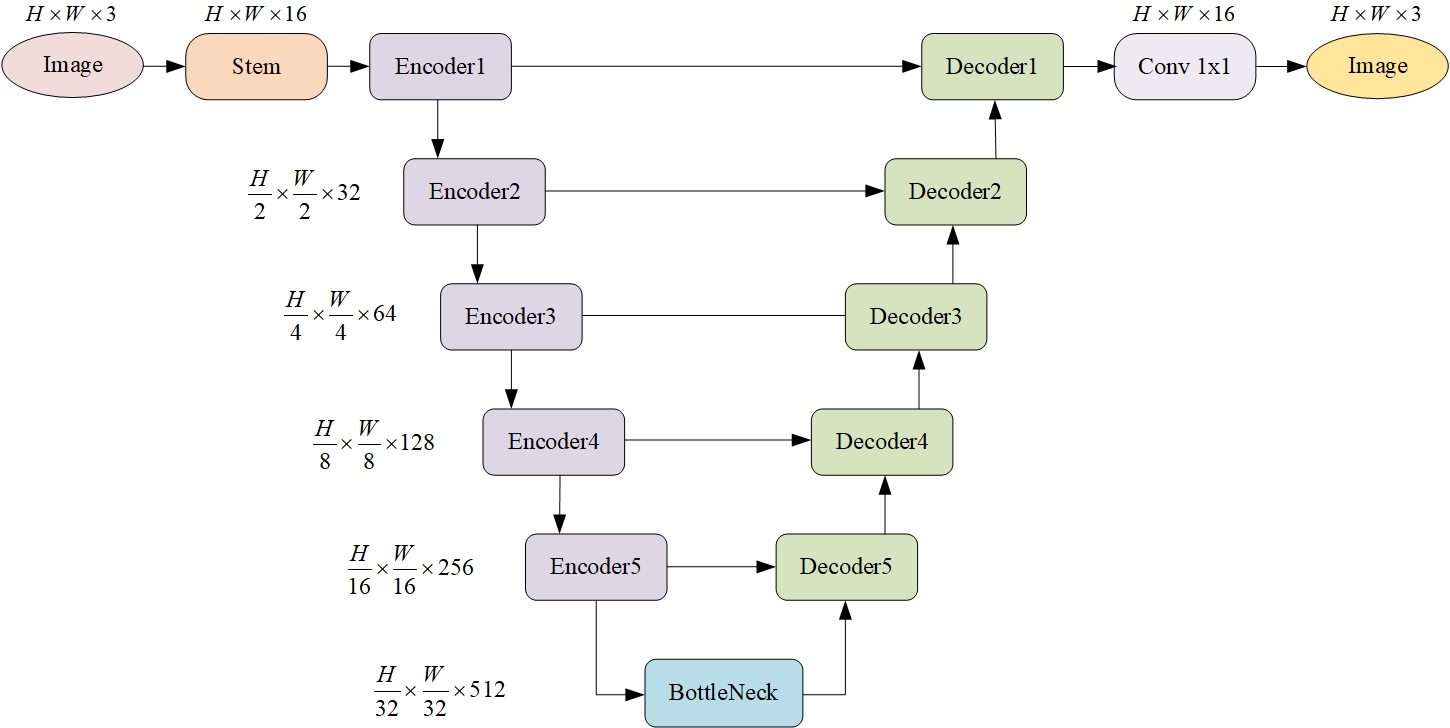
\includegraphics[width=0.8\textwidth]{picture/LLIE/My Architecture/ULite_Enhance}
			\end{center}
		\end{figure}
		
	\end{frame}
	
	\subsection{Sub-Model}
	
	\begin{frame}
		
		\begin{figure}[htbp]
			\begin{center}
				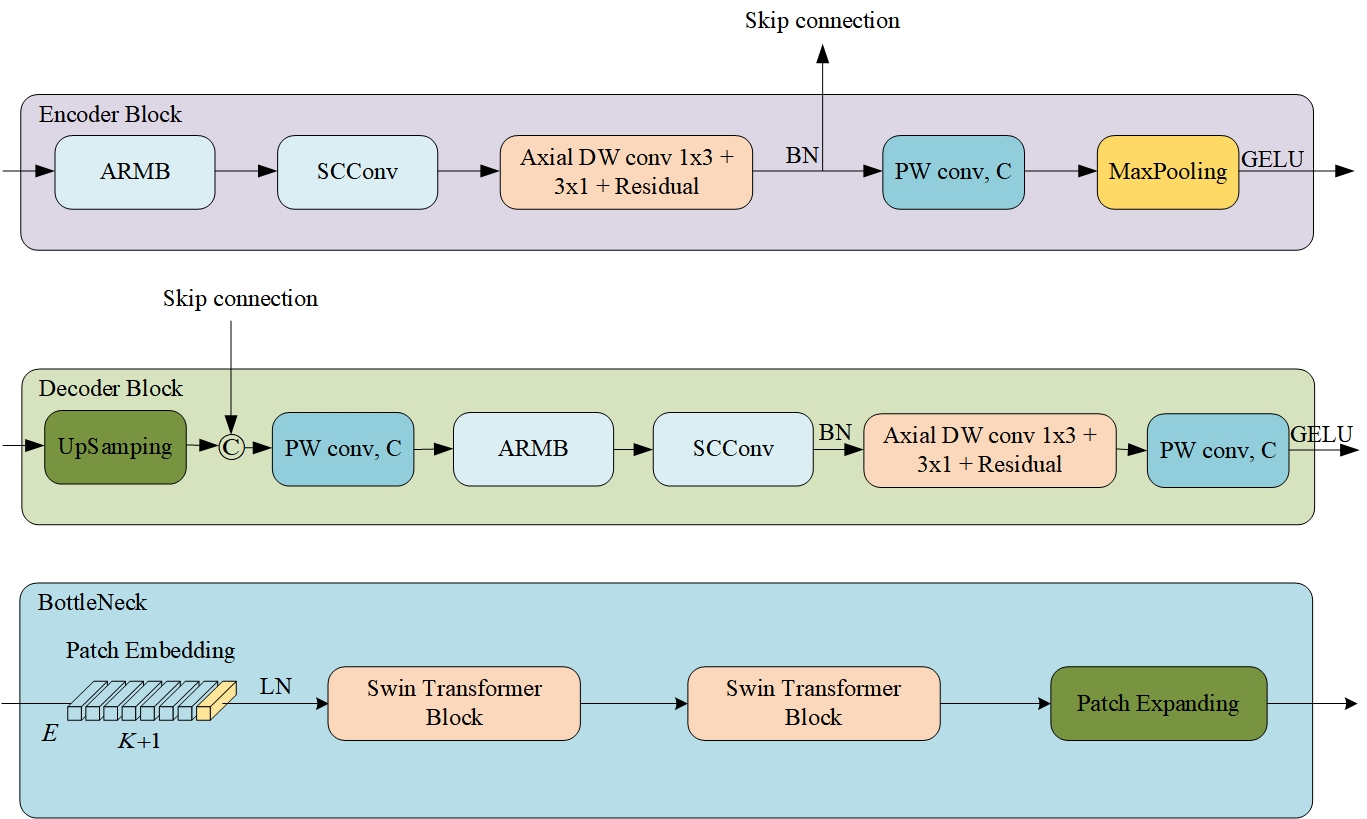
\includegraphics[width=0.8\textwidth]{picture/LLIE/My Architecture/Encoder_Decoder}
			\end{center}
		\end{figure}

	\end{frame}
	
%	\begin{frame}
%		\section{Literature Review}
%		Study hard and make progress every day. % 第一等级
%		\begin{itemize} 
%			\item Study hard and make progress every day. % 第二等级
%			\begin{itemize}
%				\item Study hard and make progress every day. % 第三等级
%				\begin{itemize}
%					\item Study hard and make progress every day. % 第四等级
%				\end{itemize}
%			\end{itemize}
%		\end{itemize}
%	\end{frame}
	
	\subsection{Swin Transformer Block}
	
	\begin{frame}
		
		\begin{figure}[htbp]
			\begin{center}
				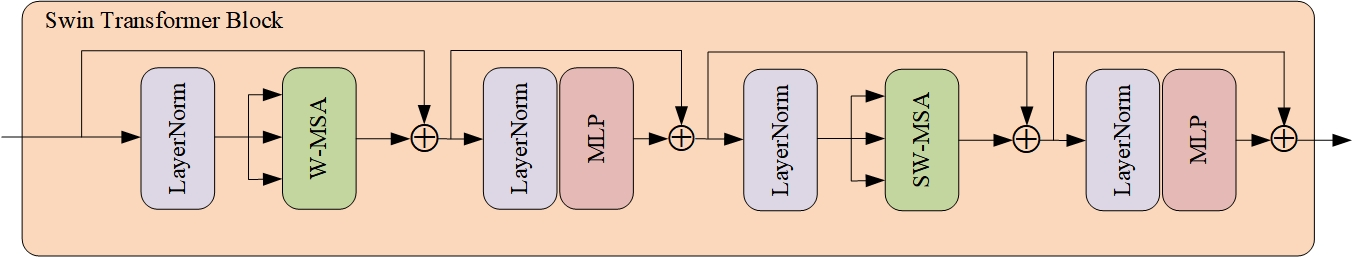
\includegraphics[width=0.8\textwidth]{picture/LLIE/My Architecture/Swin Transformer}
			\end{center}
		\end{figure}
			
	\end{frame}
	
	\section{模型贡献}
	
	\begin{frame}
		
		\begin{itemize}
			\item \textbf{贡献}
			
			\item[\checkmark] 首先,提出了一种结合卷积神经网络(CNN)和Transformer的并行架构用于弱光图像增强。
			
			% 论文提出了一种基于 GAN Loss 的模型去对结构信息建模,通过获得的结构信息指导增强。
			\vspace{.3cm}
			\item[\checkmark] 其次,提出了一个深度语义模块,该模块融合了Swin Transformer分支,使CNN分支能够有效捕获图像的长距离特征。
			
			% 从低光图像中很难提取到好的结构信息,但是论文中提出的方法提取到的结构信息会好很多,并且用于指导图像增强信息。
			
			\vspace{.3cm}
			\item[\checkmark] 最后,将深度可分离卷积融合进CNN分支中,应用于轻量级网络用于提取图像的局部特征。
		\end{itemize}	
		
	\end{frame}
	
	\section{实验计划}
	\subsection{模型构建}
	
	\begin{frame}
		
		\begin{itemize}
			\item 基于 PyTorch 进行模型的搭建、训练和评估;
			
			\item 基于 scikit-image 库计算 PSNR、SSIM 等评价指标;
		
			\item 构建 U-Net 基本架构模型;
			
			\item 实现 Swin Transformer 块中的\textcolor{blue}{LocalselfAttention}类,\textcolor{blue}{PositionEncoding}类,\textcolor{blue}{PositionEmbedding}类
		\end{itemize}

	\end{frame}
	
	\subsection{数据集}
	
	\begin{frame}
		
		% 实验的过程中,确保所有的实验在相同的硬件和软件环境下进行,并且为了确保结果的可靠性,可能需要多次运行实验并取平均值。我们主要基于 PyTorch 进行模型的搭建、训练和评估,使用 Matplotlib 库用于绘制图标和注意力图。基于scikit-image 库计算PSNR、SSIM 等评价指标。
		
		\begin{itemize} 
			\item \textbf{Low-light Dataset}
		\end{itemize}
		
		\begin{table}[!htbp]
			\centering
			\tiny
			%\resizebox{\textwidth}{!}{ %按照宽度调整调整表格大小
				\begin{tabular}{>{\centering\arraybackslash}m{3cm}|c|c|c|c}
					
					\hline
					
					\textbf{Name} & \textbf{Number} & \textbf{Format} & \textbf{Real/Syn} & \textbf{Video} \\
					
					\hline
					
					LOL\textcolor{blue}{\citep{wei2018deep}} & 500 & RGB & Real & \\
					
					SCIE\textcolor{blue}{\citep{cai2018learning}} & 4,413 & RGB & Real & \\
					
					VE-LOL-L\textcolor{blue}{\citep{jiang2019learning}} & 2,500 & RGB & Real+Syn & \\
					
					\hline
					
				\end{tabular}
				%}
			\captionsetup{font=scriptsize} %设置标题字体与表格字体一致
			\caption{\label{tab: Paired_training_datases}
				Summary of paired training datasets. 'Syn' represents Synthetic.} %表格的标题
			
		\end{table}
	\end{frame}
	
	\subsection{训练}
	
	\begin{frame}
		\begin{itemize}
			\item \textbf{Train}
			
			\checkmark Baseline Model
			% 基线模型: 首先,训练基线模型(即完整的并行模型,包含完整的CNN 和Transformer 分支)。
			
			\checkmark Ablation Study
			% 消融研究: 接着,训练去除Transformer 分支的模型,以进行消融实验。
		\end{itemize}
		
		\begin{itemize}
			\item \textbf{Performance Evaluation}
			
			%\checkmark MSE
			% 均方误差
			
			\checkmark PSNR
			% 峰值信噪比
			
			\checkmark SSIM
			% 结构相似性指数
			
			\checkmark LPIPS
			% 感知图像质量评估
		\end{itemize}
		
		\begin{itemize}
			\item \textbf{Loss Function}
			
			\checkmark 休伯损失函数和SSIM损失函数
			\vspace{-.3cm}
				\begin{equation}
					L_{loss} = \alpha J_{Huber}(\delta) + \beta \mathcal{L}^{\text{SSIM}}(P)
				\end{equation}
				
			\checkmark 休伯损失函数,SSIM损失函数,Perceptual损失函数(耗费更多训练时间)
			\vspace{-.3cm}	
				\begin{equation}
					L_{loss} = \alpha J_{Huber}(\delta) + \beta \mathcal{L}^{\text{SSIM}}(P) + \gamma \ell_{feat}^{\phi,j} (\hat{y},y)
				\end{equation}
		\end{itemize}
				
	\end{frame}
	
	
	
	\begin{frame}[plain,c]
		\begin{center}
			\Huge Thank you !
		\end{center}
	\end{frame}
	
%	\appendix
%	\begin{frame}[allowframebreaks]{References}
%		\tiny
%		%\bibliographystyle{unsrt}
%		\bibliographystyle{elsarticle-harv}
%		\bibliography{reference}
%		%\bibliographystyle{plainnat}
%	\end{frame}
	
\end{document}
